\documentclass{article}

\usepackage[sglblindworkshop, final]{neurips_2026}
\workshoptitle{Predictive AI Evaluation Competition}

\usepackage[utf8]{inputenc}
\usepackage[T1]{fontenc}
\usepackage{hyperref}
\hypersetup{hidelinks}
\usepackage{url}
\usepackage{booktabs}
\usepackage{array}
\usepackage{amsfonts}
\usepackage{amsmath}
\usepackage{nicefrac}
\usepackage{microtype}
\usepackage{xcolor}
\usepackage{graphicx}

\title{LLM priors on item difficulty and subject ability for predicting AI benchmark outcomes}

\author{
  Stanley Mei \\
  Stanford University \\
  \texttt{smei@stanford.edu}
}

\begin{document}

\maketitle

% Abstract -- drafted by Claude (2026-10-21).
\begin{abstract}
  Predicting whether an AI system will solve a task, without running it, could make evaluation cheaper. The Predictive AI Evaluation Competition tests such predictors on hidden benchmarks: for an AI system (a subject) and an item, they give a probability of success from the subject's recorded fields, the item's text and the labels acquired so far for that subject and others in the same draw. My entry chains small Bayesian models: a normal prior on the subject's ability, updated on its labels, and item difficulties pooled from other subjects' labels. Claude Opus 5.5 supplies two further priors, a rating of each item's difficulty and a guess of each subject's success rate, each calibrated on public data and trusted only as far as a worst-case analysis allows. On rated items, with each public benchmark held out in turn, the ratings improved Brier ALC by 0.0144 (SE 0.0011) and the guesses by a further 0.0135 (SE 0.0013). On one hosted draw, the guesses lowered the Brier score before any label from 0.25 to 0.180. Claude may have seen results on the public benchmarks in training, so the gains could be smaller on new ones.
\end{abstract}

% Section 1 -- drafted by Claude (2026-10-21), revised after review.
\section{Introduction}\label{sec:intro}

The Predictive AI Evaluation Competition \citep{truong2026paiec} scores predictors on benchmarks they have never seen. For an AI system (a subject) and an item of a hidden benchmark, the predictor gives the probability that the subject succeeds, without running it. It starts from the subject's recorded fields and the item's text. Codabench scores each upload on a fresh random draw of subject--benchmark pairs (8 or 9 in each draw I saw) as formative feedback. At budgets of 1 to 31 labels the predictor also sees the subject's outcomes on other items of that benchmark, with the labels of other subjects in the same draw. The Brier ALC (area under the learning curve, Eq.~\eqref{eq:alc}) averages the Brier scores at six budgets from 0 to 31 labels and puts 70\% of its weight on budgets of 7 labels or fewer. This is a small instance of predictable AI in the sense of \citet{zhou2026predictable}.

Item response models have been applied to AI evaluation data \citep{lalor2016building,martinezplumed2019irt,rodriguez2021evaluation} and can estimate a model's score from a few items \citep{polo2024tinybenchmarks,truong2025reeval}; \citet{truong2025reeval} also predict a new item's difficulty from its content, with a predictor fit to responses on other items. Without such a predictor, these methods need responses on the same items, and at the start of a hidden benchmark there are none. \citet{zhang2025benchmark} found that a random sample with a regression adjustment beats most benchmark-prediction methods, and that when new models are more accurate than those seen before, none of these methods consistently beats a plain average over a random sample. Estimating difficulty from item text alone is an old problem in education \citep{benedetto2023survey}, and LLM judgments of the difficulty of human test items match measured difficulty only weakly to moderately \citep{chrzan2026consensus,li2026llms}.

I built the entry as a chain of small Bayesian models and decided most additions by a rule written before its test (Appendix~\ref{app:rules} lists the exceptions). V1 places a normal prior on a subject's ability, centered on a score from the subject's metadata, and updates it on a grid; V2 pools item difficulties from the labels of other subjects in the same draw. V3 keeps V2 but drops the metadata score from the prior, so that it predicts 0.5 before the first label. Most of the offline gain came from the two LLM inputs added last: V4 uses Claude Opus 5.5's rating of each item's difficulty as a prior, and V5, the final entry, adds the same model's guess of how often the subject succeeds on the benchmark. Both inputs are calibrated on public data and enter with a trust level chosen to limit the loss if they turn out to be wrong. Because Claude may have seen these public benchmarks in training, the offline gains may overstate what transfers to new ones (Section~\ref{sec:limitations}). The contributions are:
\begin{itemize}
  \item a local harness that simulates the scoring protocol and whose ALC computation reproduces all 68 per-pair scores I kept from Codabench, together with the rules fixed before each test and the ideas that failed (Sections~\ref{sec:data} and~\ref{sec:analysis}, Appendix~\ref{app:rules});
  \item two ways to use an LLM inside a Bayesian predictor, as a gated prior on item difficulty and as a prior on subject ability, which improve offline Brier ALC on rated items by 0.0144 (SE 0.0011) and a further 0.0135 (SE 0.0013) (Sections~\ref{sec:method} and~\ref{sec:results});
  \item a submission that calls an LLM API during hosted scoring despite hidden program output, no package installation and workers that restart at every budget (Section~\ref{sec:llm});
  \item an account of what single formative draws can show: metadata priors helped offline but hurt at budget 0 on all three hosted draws, and the final entry's budget-0 Brier fell to 0.180 from the 0.25 of a constant 0.5 (Section~\ref{sec:results}).
\end{itemize}

% Section 2 -- drafted by Claude (2026-10-10), revised after a fact check (2026-10-11); V5 rules added 2026-10-21.
\section{Task, data and local evaluation}\label{sec:data}

The predictor outputs the probability that a subject succeeds on an item. A subject is an AI system defined by its model, evaluation harness, harness version and reasoning effort; the items come from benchmarks in the competition's private test pool \citep{truong2026paiec}. Codabench \citep{xu2022codabench} scores a draw of subject--benchmark pairs. Each pair's items are split in half: an acquisition stream that supplies the labels and an evaluation set that is scored after budgets of $b \in \{0, 1, 3, 7, 15, 31\}$ acquired labels. With $B_b$ the pair's Brier score \citep{brier1950} at budget $b$, the pair's Brier ALC (area under the learning curve) is
\begin{equation}
  \mathrm{ALC} = 0.1\,B_0 + 0.2\,(B_1 + B_3 + B_7 + B_{15}) + 0.1\,B_{31},
  \label{eq:alc}
\end{equation}
and the score of a submission is the mean over pairs. Lower is better. At each budget the predictor receives the labels acquired so far for every pair in the draw (none at budget 0), so when a draw puts several subjects on one benchmark, it can use the other subjects' labels. None of my uploads included a labeling policy, and the platform acquired labels at random. Each upload gets formative feedback: its score on one draw of pairs (8 or 9 for me), drawn afresh each time, with per-budget Brier tables.

\paragraph{Data.}
I trained and tested on the public measurement-db \citep{measurementdb2026} at revision \texttt{bc8204d8}; the only other training data are the LLM difficulty ratings and subject guesses described in Section~\ref{sec:method}. Because the competition scores binary outcomes, I kept an item only if its declared response scale is $\{0,1\}$. This drops MMDocRAG \citep{dong2025mmdocrag}, graded on a 26-level scale, and 271 MathArena items graded on an interval scale (Appendix~\ref{app:harness}). What is left is 10,361 items, 229 subjects and 225,764 responses on five benchmarks: MathArena \citep{balunovic2025matharena}, Multi-SWE-bench \citep{zan2025multiswe}, REAL \citep{garg2025real}, ResearchCodeBench \citep{hua2025researchcodebench} and SWE-rebench \citep{badertdinov2025swerebench} (Table~\ref{tab:data}).

\begin{table}[h]
  \caption{Public training data after the binary-scale filter. Responses include repeated trials; mean label is the share equal to 1. Pairs: pairs with 80 to 1,000 items (default setting, per seed). Rated items: items with an LLM rating (1,379 items share 1,049 ratings; on MathArena, 696 items cover 366 problems). Rated pairs: pairs with at least 40 rated items (rated setting, per seed). The total row counts distinct subjects.}
  \label{tab:data}
  \centering
  \small
  \setlength{\tabcolsep}{4pt}
  \begin{tabular}{lrrrrrrr}
\toprule
Benchmark & Items & Responses & Subjects & Mean label & Pairs & Rated items & Rated pairs \\
\midrule
MathArena & 1,484 & 89,482 & 95 & 0.67 & 81 & 696 & 65 \\
Multi-SWE-bench & 2,126 & 57,975 & 82 & 0.15 & 54 & 400 & 70 \\
REAL & 233 & 4,449 & 33 & 0.36 & 26 & 233 & 32 \\
ResearchCodeBench & 212 & 6,784 & 31 & 0.36 & 31 & 50 & 31 \\
SWE-rebench & 6,306 & 67,074 & 1 & 0.48 & 0 & -- & -- \\
\midrule
Total & 10,361 & 225,764 & 229 & & 192 & 1,379 & 198 \\
\bottomrule
\end{tabular}

\end{table}

\paragraph{Local evaluation.}
To compare predictors offline I wrote a harness that simulates the hosted protocol on the public data. Each fold holds out one benchmark: the predictor is fit on the other four and scored on pairs from the held-out one. Each subject with enough items on the held-out benchmark forms a pair, whose items are shuffled with a seeded generator and split in half. Labels are acquired in rounds (Appendix~\ref{app:harness}) with the default random rule of the competition's starting kit, and at each budget the predictor is scored on every recorded response of the evaluation items. Recomputing each pair's ALC from the per-budget Brier tables of my Codabench feedback reproduces the reported value to within $10^{-6}$ for all 68 pair results I kept. Appendix~\ref{app:harness} gives the details and the check's limits.

I compare predictors in three settings. The \emph{default} setting follows the rules' minimum of 80 items per pair and caps pairs at 1,000 items, the platform's limit for a whole draw; it gives 192 pairs per seed, with 265 items on average. The \emph{hidden-sized} setting imitates the smaller pairs of a Codabench draw, where the 8 or 9 pairs of each draw I saw shared at most 1,000 subject--item combinations: it samples at most 400 items of the held-out benchmark and keeps pairs with at least 60, about 157 pairs per seed with 153 items on average. For the \emph{rated} setting, which tests the LLM inputs, I kept only items with an LLM rating and pairs with at least 40 of them (198 pairs per seed). I lowered the minimum below the rules' 80 in the last two settings to keep enough pairs. In any setting a pair can also be given the labels of $K$ partner pairs on the same benchmark, and I give $K$ with each result.

All runs use seeds 0, 1 and 2, which set the split, the stream order and the partners but not the fitted predictor. A comparison reports $\Delta = \mathrm{ALC}(\text{candidate}) - \mathrm{ALC}(\text{reference})$, averaged over all seeds' pair results, matched on seed and pair, so $\Delta < 0$ favors the candidate. Its standard error treats each subject--benchmark pair as one cluster across the seeds (CR0, Appendix~\ref{app:harness}). Appendix~\ref{app:rules} lists each test's rule, written before its run, and the choices made without a rule.

% Section 3 -- drafted by Claude (2026-10-11), revised after checks (2026-10-11, 2026-10-21); V5 added 2026-10-21.
\section{Method}\label{sec:method}

My baseline (Codabench 954621) predicts $(4p_0 + k)/(4 + n)$ for a pair with $k$ successes in $n$ acquired labels, where $p_0$ is a prior success rate from the subject's metadata: a beta--binomial update with prior strength 4 (Appendix~\ref{app:model}). V1 to V5 build on one another; V5 is the final entry, and Table~\ref{tab:formative} gives the Codabench submission of each version.

Throughout, $\theta_s$ is subject $s$'s ability on the benchmark being predicted. Labels on other benchmarks are not used, and item difficulties are centered within each benchmark, so the benchmark's mean difficulty is absorbed into $\theta_s$. I write $\sigma$ for the logistic function and $\kappa(v) = \sqrt{1 + \pi v/8}$ for the factor of the probit approximation $\mathbb{E}[\sigma(x)] \approx \sigma(\mu/\kappa(v))$ for $x \sim \mathcal{N}(\mu, v)$ \citep{mackay1992evidence}.

\subsection{Ability prior and grid posterior (V1, V3)}
V1 gives every item of a pair the success probability $\sigma(\theta_s)$, with a normal prior $\theta_s \sim \mathcal{N}(m_s, s_\theta^2)$, $s_\theta = 1.5$, so the success rate is logit-normal. The prior mean is $m_s = \lambda\,(g(s) - \bar g)$, clipped to $[-6, 6]$, where $g(s)$ is the subject part of the baseline's metadata regression (release date, a ``thinking'' variant flag and the provider, plus a shrunken residual for subjects seen in training; Appendix~\ref{app:model}) and $\lambda$ is a scale. After $k$ successes in $n$ own labels,
\[
  p(\theta \mid \text{labels}) \propto \mathcal{N}(\theta; m_s, s_\theta^2)\, \sigma(\theta)^k\, \sigma(-\theta)^{n-k},
\]
which I evaluate on a fixed grid and summarize by the posterior mean of $\sigma(\theta)$, an expected-a-posteriori estimate \citep{bock1982eap}. V1 used $\lambda = 0.5$, although $\lambda = 1$ was better offline by 0.0016 (SE 0.0004): in a scenario analysis that is not in the repository, the half-strength prior had about a third of the full prior's worst-case loss when metadata do not carry over, with the same average. Two of its scenarios were modeled on the baseline's formative per-budget curve; the choice held without them. For V3 I set $\lambda = 0$; as no labels are passed at budget 0, every prediction there is exactly 0.5. This is the one model setting I chose directly from formative feedback, and offline it was worse (Section~\ref{sec:data}); the other use of feedback was the choice between V4 and V5 (Section~\ref{sec:results}). I tried one alternative to $s_\theta = 1.5$: at $\lambda = 1$, $s_\theta = 1.75$ scored $+0.0016$ (SE 0.0002) worse, and I kept 1.5.

\subsection{Item pooling (V2)}
In V2 items differ in difficulty. A Rasch model \citep{rasch1960} gives
\begin{equation}
  P(y_{si} = 1) = \sigma(\kappa_0\theta_s - z_i), \qquad z_i \sim \mathcal{N}(0, \tau^2), \qquad \kappa_0 = \kappa(\tau^2),
  \label{eq:rasch}
\end{equation}
with $\tau = 2$ (not tuned) and $\kappa_0 \approx 1.60$; a larger $z_i$ is a harder item. With $\phi_s = \kappa_0\theta_s$ this is the organizers' $\sigma(\phi_s - z_i)$ \citep{truong2025reeval}. The factor $\kappa_0$ keeps $\theta$ on V1's scale: by the probit approximation, averaging over an unknown difficulty gives back $\sigma(\theta_s)$, with an error of at most 0.0101 for $\theta_s \in [-6, 6]$.

A difficulty can only be learned from other subjects' labels on the same item, which the predictor sees when a draw puts several subjects on one benchmark. In my own formative draws few pairs shared a benchmark, so pooling seldom had partner labels to use. I estimate difficulties with a two-stage calibration \citep{ban2001online,truongkoyejo2026aims}: each partner label becomes an observation of the item's difficulty, given that partner's ability estimated from its \emph{other} labels, and the observations are combined with the prior on $z_j$ into a posterior mean $\hat z_j$ and variance $\omega_j^2$ (Appendix~\ref{app:model}). The target subject's labels on items with a known difficulty then enter its likelihood through $\hat z_j$ and $\omega_j^2$, its other labels enter as in V1, and the prediction for an item averages $\sigma(\kappa_0\theta - z)$ over the posteriors of $\theta$ and of the item's difficulty. Items carry no identifier, so I match them across subjects by their content and features. With no partner labels, V2 gives exactly V1's predictions.

\subsection{LLM difficulty ratings and the gate (V4)}
For V4 I also had Claude Opus 5.5 \citep{anthropic2026opus55} rate how hard each item is. The rater sees the item's content and features with a fixed rubric (Appendix~\ref{app:prompt}), is told not to solve the item, and returns one integer from 1 (almost every AI system released in 2023--2026 completes it) through 5 (about half do) to 10 (almost none do); a refusal or a value outside 1--10 counts as unrated. Offline I had it rate 1,049 public items, one per problem, which through shared content cover the 1,379 rated items of Table~\ref{tab:data}, at an estimated cost of \$12.08. Against Rasch difficulties fitted separately on each benchmark to all subjects' public responses (Appendix~\ref{app:model}), the Spearman correlations were 0.82 (366 rated problems), 0.28 (400 items), 0.44 (233) and 0.77 (50) on MathArena, Multi-SWE-bench, REAL and ResearchCodeBench. These benchmarks are public, and the rater may partly remember how hard their items are.

A rated item $j$ with rating $r_j$ gets the prior
\begin{equation}
  z_j \sim \mathcal{N}\bigl(\beta_t\,(r_j - \bar r),\ \rho_t^2\bigr),
  \nonumber
\end{equation}
which replaces the prior $\mathcal{N}(0, \tau^2)$ of Eq.~\eqref{eq:rasch} in the second stage and is used directly when the item has no partner labels; this is an explanatory item model in the sense of \citet{deboeck2004explanatory}. Here $\bar r$ is the mean rating of the rated items already labeled on the benchmark, by the target subject or by partners. Ratings thus enter only through their difference from that mean, and their absolute level is never used; until a rated item is labeled, and so always at budget 0, they have no effect. The slope $\beta$ and residual standard deviation $\rho$ come from a regression of the Rasch difficulties on the ratings, pooled within benchmarks: $\beta = 0.788$ and $\rho = 1.904$ for the submission, which uses all four rated benchmarks; the offline evaluation refits them without the held-out benchmark. A trust level $t \in [0, 1]$ interpolates between V3's prior and the fitted regression,
\begin{equation}
  \beta_t = t\beta, \qquad \rho_t^2 = \tau^2 - t^2 \max(\tau^2 - \rho^2, 0).
  \label{eq:trust}
\end{equation}
Because $\rho < \tau$ in every fit, $t = 0$ gives V3 and $t = 1$ gives $(\beta, \rho)$; because $\rho$ is close to $\tau$, $t$ acts almost only through the slope. I chose $t = 0.5$ ($\beta_t = 0.394$, $\rho_t = 1.976$) with a rule fixed before the run: it had the smallest worst-case regret over real, half-noisy and shuffled ratings (Section~\ref{sec:results}). A trust level's regret in a scenario is its Brier ALC minus that of the best trust level in the same scenario; half-noisy ratings keep each item's rating with probability 1/2 and otherwise take the rating of a random other item of the benchmark. With these values, after one solved label on an item rated 3, an item rated 8 gets 0.417 under V4 and 0.647 under V3.

Ratings that point the wrong way hurt. Offline, V4 without the gate was worse than V3 by 0.027 Brier ALC with the ratings reversed and by 0.0065 with them shuffled, and with the gate by 0.011 and 0.0048. The gate makes V4 predict as V3 whenever the benchmark has at least three labels on rated items, both outcomes occur among them, and the failed items have the lower mean rating. During scoring V4 requests ratings of the hidden items from the API with the same prompt; without a working key it predicts exactly as V3 (Section~\ref{sec:llm}).

\subsection{Guessed subject priors (V5)}
Ratings say nothing at budget 0, and on all three hosted draws scored with a metadata prior, the budget-0 predictions did worse than a constant 0.5 (Section~\ref{sec:results}). V5 instead asks Claude how strong the subject is. The request shows the subject's recorded fields, exactly as the platform passes them, and one item of the benchmark as an example, and asks what percentage of the benchmark's items the subject completes (Appendix~\ref{app:prompt}); it names no benchmark and contains no labels. During scoring the example is whichever item of the pair is predicted first. Before building V5 I checked, with a rule fixed in advance, whether Claude knows subject strength at all. With three example items per benchmark, the Pearson correlation between the logit of its guess and Rasch ability, computed within each benchmark and averaged over the four, was 0.818 (0.957 on MathArena, 0.767, 0.661 and 0.886 on the others). V1's metadata score reached 0.611 on the same measure. The single-example guesses that V5 uses reach 0.771.

The guess $q_s$ enters through a calibration. On the public pairs, an ordinary least-squares fit of the logit of each pair's success rate on $\operatorname{logit} q_s$, both clipped to $[0.01, 0.99]$, gives an intercept $a_g$, a slope $c_g$ and a residual standard deviation $s_g$. A subject with a guess then gets
\begin{equation}
  \theta_s \sim \mathcal{N}\bigl(t_g\,(a_g + c_g \operatorname{logit} q_s),\ (1 - t_g^2)\,s_\theta^2 + t_g^2 s_g^2\bigr),
  \label{eq:guessprior}
\end{equation}
with $q_s$ clipped to $[0.01, 0.99]$ and the mean to $[-6, 6]$ as in V1. This replaces V4's $\mathcal{N}(0, s_\theta^2)$ for the target subject and for every partner whose labels are pooled. The guess trust $t_g$ interpolates as in Eq.~\eqref{eq:trust}: $t_g = 0$ is V4 and $t_g = 1$ trusts the calibration fully. A subject without a guess keeps V4's prior. I chose $t_g = 0.75$ by the same minimax-regret rule as the rating trust, over real guesses, shuffled guesses and every guess moved by $\pm 1$ on the logit scale (Section~\ref{sec:results}). The submission's calibration uses all four rated benchmarks (204 pairs): $a_g = 0.040$, $c_g = 0.851$, $s_g = 0.811$, which gives the prior $\mathcal{N}(0.030 + 0.639 \operatorname{logit} q_s,\ 1.164^2)$. At budget 0 every item of a pair gets the prior mean of $\sigma(\theta_s)$: a guess of 10\% gives 0.25, 30\% gives 0.40 and 90\% gives 0.76, closer to 0.5 than the guesses themselves.

% Section 4 -- drafted by Claude (2026-10-21), revised after review.
\section{Calling an LLM during scoring}\label{sec:llm}

V4 and V5 call the Anthropic API while Codabench scores them. The rules limit network access during scoring to ``approved inference APIs'' without naming them; after a probe had shown the API reachable and after my V4 upload, the organizers confirmed to me that Anthropic's API is one of them. Participants cannot see the platform's logs, and I learned how it behaves from probe uploads (Appendix~\ref{app:engineering}). The platform does not install the packages in \texttt{requirements.txt}, so the submission talks to the API through Python's standard library, sending the same request body and headers as the official client. It also starts fresh worker processes at every budget, but files written in the submission folder stay there. The submission therefore keeps every reply in a file in its own folder, one per item for ratings and one per subject and benchmark for guesses, which all workers share, with lock files so that each request is paid for once. A prediction waits at most 4 seconds for pending requests; timed from my machine, a guess took 1.4 to 3.1 seconds and a rating 1.3 to 1.7 seconds, and V5 sends guesses first because they are used from budget 0. At most 1,000 billed attempts are made per run.

Because a single exception would fail the whole run, no failure raises an error; each falls back to a simpler model. A missing rating gives that item V3's treatment, and a missing guess gives that subject V4's prior. With no key, or no usable API, V5 predicts exactly as V3: run through my harness without a key, it reproduced V3 on all 576 pair results of the default setting. The key never enters the repository; I add it to a private copy of the zip with a script that checks it first, and it belongs to a workspace with a [TO CONFIRM: \$50] spending limit used for nothing else. The V4 run cost \$9.49, billed; [TO CONFIRM: V5 run cost, billed]. The model is \texttt{claude-opus-5-5} at low effort with JSON-schema output, and the request allows a server-side fallback to \texttt{claude-opus-4-8}. The submission does not record which model answered, but offline all 1,473 saved replies (1,049 ratings and 424 guesses) came from Opus 5.5. Replies vary from call to call and the hosted ones stay in the scoring folder, which participants cannot read, so a rerun will not reproduce the feedback exactly.

% Section 5 -- drafted by Claude (2026-10-21), revised after review. Numbers from scripts/report_results.py.
\section{Results}\label{sec:results}

\paragraph{Offline.}
Table~\ref{tab:offline} follows the versions through the three settings of Section~\ref{sec:data}. In the default setting V1 scored about the same as the baseline ($-0.0003$, SE 0.0011), and setting $\lambda$ to 0 for V3 cost $+0.00300$ (SE 0.00047). In the hidden-sized setting, pooling difficulties from one partner pair helped a little on each of the four benchmarks with partner pairs ($-0.00116$, SE 0.00015), assuming, as my harness does, that each pair's items are split independently; with one split shared by every subject on a benchmark the gain was $-0.00007$ (SE 0.00005). The large offline gains came from the two LLM inputs, testable only in the rated setting. The difficulty ratings gave $-0.0144$ (SE 0.0011), $-0.0144$ (SE 0.0009) and $-0.0141$ (SE 0.0008) with one and two partner pairs, and $-0.0140$ (SE 0.0010) and $-0.0097$ (SE 0.0007) with only 90\% or 70\% of items rated. The guesses gave another $-0.0135$ (SE 0.0013), $-0.0132$ (SE 0.0012) with one or two partner pairs, and beat V4 on each held-out benchmark ($-0.0077$ on MathArena, $-0.0217$ on Multi-SWE-bench, $-0.0101$ on REAL and $-0.0109$ on ResearchCodeBench). The submission folders gave a similar gain in-sample (Appendix~\ref{app:engineering}).

\begin{table}[t]
  \caption{Offline Brier ALC (lower is better) in three settings, pooled over seeds 0--2. $\Delta$ is a row's score minus the score of the row above it on the same pair results (negative favors the row); the SE treats each subject--benchmark pair as a cluster. Blocks use different pairs, so their scores and differences cannot be added. V3 is worse than V1 and V2 offline in every block where they meet; I adopted it because of formative feedback (Appendix~\ref{app:rules}).}
  \label{tab:offline}
  \centering
  \small
  \begin{tabular}{lrrr}
\toprule
Predictor & Pair results & Brier ALC & $\Delta$ to row above (SE) \\
\midrule
\multicolumn{4}{l}{\emph{Default setting, $K = 0$}} \\
\quad Baseline & 576 & 0.2161 & -- \\
\quad V1 ($\lambda = 0.5$) & 576 & 0.2158 & $-0.0003$ (0.0011) \\
\quad V3 ($\lambda = 0$) & 576 & 0.2188 & $+0.00300$ (0.00047) \\
\addlinespace
\multicolumn{4}{l}{\emph{Hidden-sized setting, $K = 1$}} \\
\quad V1 ($\lambda = 0.5$) & 471 & 0.1959 & -- \\
\quad V2 ($\lambda = 0.5$, pooling) & 471 & 0.1948 & $-0.00116$ (0.00015) \\
\quad V3 ($\lambda = 0$, pooling) & 471 & 0.1993 & $+0.00459$ (0.00055) \\
\addlinespace
\multicolumn{4}{l}{\emph{Rated setting, $K = 0$}} \\
\quad V3 & 594 & 0.2074 & -- \\
\quad V4 (ratings, $t = 0.5$, gate) & 594 & 0.1930 & $-0.0144$ (0.0011) \\
\quad V5 (V4 + subject guesses, $t_g = 0.75$) & 594 & 0.1795 & $-0.0135$ (0.0013) \\
\bottomrule
\end{tabular}

\end{table}

Most of V5's gain comes at the first budgets (Figure~\ref{fig:budgets}). At budget 0 V4 predicts 0.5 everywhere and scores 0.2500, against V5's 0.2037. Weighted as in Eq.~\eqref{eq:alc}, budgets 0 and 1 give 74\% of V5's gain over V4 and budget 3 another 17\%, and by budget 31 the two curves meet.

\begin{figure}[t]
  \centering
  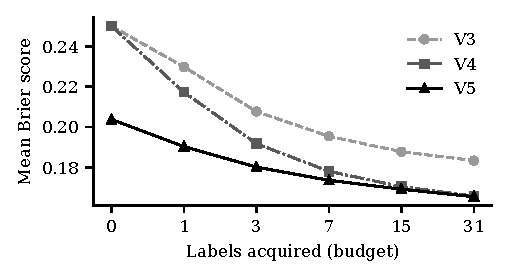
\includegraphics[width=0.56\linewidth]{figures/budgets}
  \caption{Mean Brier score at each budget in the rated setting with no partner pairs (594 pair results; budgets on a $\log_2(1 + b)$ axis). V4's ratings act from budget 1 on and grow with the labels; V5's guesses act from budget 0 and matter most before the first few labels.}
  \label{fig:budgets}
\end{figure}

I chose both trust levels to limit the damage if the LLM inputs do not transfer. At trust levels 0, 0.25, 0.5, 0.75 and 1, the worst-case regret was 0.0188, 0.0096, 0.0065, 0.0142 and 0.0236 for the rating trust $t$ and 0.0148, 0.0094, 0.0049, 0.0013 and 0.0108 for the guess trust $t_g$. At $t_g = 0.75$, V5 still beat V4 when the held-out benchmark's guesses were shuffled among its subjects ($-0.0024$, SE 0.0020), raised by one logit ($-0.0045$, SE 0.0013) or lowered by one ($-0.0126$, SE 0.0019). These scenarios are milder than what happened to the metadata priors on Codabench. Shuffling keeps the benchmark's average level: Multi-SWE-bench, which gives 57\% of V5's gain, still gained 0.0107 with shuffled guesses, while MathArena lost 0.0081. No scenario in the rule combined a shuffle with a shift or reversed the guesses; computed afterwards, either case makes V5's budget-0 Brier worse than 0.25, by 0.006 for shuffled guesses moved up one logit and by 0.021 for reversed ones.
\paragraph{Formative feedback.}
Table~\ref{tab:formative} lists the upload of each version; the probes of Appendix~\ref{app:engineering} are left out. Each row comes from its own draw (Section~\ref{sec:data}), so differences between rows mix version and draw, and I use two quantities that depend less on the draw. A version that predicts one value $p$ for every item of a pair at budget 0 has Brier score $(p - \bar y)^2 + \bar y(1 - \bar y)$ and calibration error $|p - \bar y|$, where $\bar y$ is the pair's success rate; the Brier score minus the squared calibration error recovers the floor $\bar y(1-\bar y)$, which I subtract from the score to discount easy draws. And since V3 and V4 predict exactly 0.5 at budget 0, their budget-0 Brier is 0.25 on any draw, a fixed reference for later versions.

\begin{table}[t]
  \caption{Formative Codabench results, each a single draw (UTC+8 dates). Score: mean Brier ALC over the draw's pairs. Floor: the draw's mean $\bar y(1-\bar y)$ recovered from the budget-0 rows, so score $-$ floor discounts easy draws (SE over pairs; approximate for V5, whose first budget-0 predictions may have come before the guess arrived). The first row is a constant 0.5.}
  \label{tab:formative}
  \centering
  \small
  \setlength{\tabcolsep}{4pt}
  \begin{tabular}{llcrrrr}
\toprule
Codabench & Date & Version & Pairs & Score & Budget-0 Brier & Score $-$ floor (SE) \\
\midrule
951242 & 2026-09-29 & constant 0.5 & 8 & 0.2500 & 0.250 & 0.078 (0.022) \\
954621 & 2026-10-01 & Baseline & 9 & 0.2322 & 0.298 & 0.048 (0.013) \\
958131 & 2026-10-03 & V1 & 9 & 0.2025 & 0.283 & 0.036 (0.011) \\
963204 & 2026-10-06 & V2 & 8 & 0.1877 & 0.303 & 0.045 (0.011) \\
963789 & 2026-10-06 & V3 & 9 & 0.1559 & 0.250 & 0.034 (0.008) \\
968769 & 2026-10-08 & V4 & 8 & 0.1704 & 0.250 & 0.031 (0.011) \\
1005477 & 2026-10-20 & V5 & 8 & 0.1408 & 0.180 & 0.009 (0.007) \\
\bottomrule
\end{tabular}

\end{table}

The baseline, V1 and V2 all scored worse than 0.25 at budget 0 (0.298, 0.283 and 0.303), although offline they had been below it (0.244 and 0.238 for the baseline and V1 in the default setting, 0.232 for V2 in the hidden-sized one). On the hidden benchmarks their metadata priors put budget-0 predictions further from the pairs' success rates than 0.5 was, so I switched to V3. V5's budget-0 Brier was 0.180 on 8 pairs, below 0.25 on 6 of them. By the rule I committed before uploading it (Appendix~\ref{app:rules}), V5 replaced V4 as the final entry. Its score net of the floor, 0.009 (SE 0.007), is the lowest of all uploads; V4's was 0.031 (SE 0.011). With one draw per version and standard errors this wide, I read the formative results as consistent with the offline ones, not as a separate measure.

% Section 6 -- drafted by Claude (2026-10-21), revised after review.
\section{What did not work}\label{sec:analysis}

Three ideas failed their rules (Appendix~\ref{app:rules}). Ridge regressions from two sentence-embedding models to Rasch difficulty ranked items within a benchmark about as well as word counts did (Spearman 0.20 to 0.51), but on a held-out benchmark the correlation fell to between $-0.06$ and $0.04$. Question groups gave a subject its own offset for each group of items sharing their first feature field, such as a math competition, a website or a paper. Their net effect was small ($-0.0004$, SE 0.0004): they helped where that field names such a group, but on Multi-SWE-bench it names the programming language, and there they hurt by more than the rule allowed. I did not redefine the groups after seeing this, since that would have chosen the rule from the result.

The agent rule set $\lambda$ to 0 for subjects run inside an agent harness, on the idea that the harness matters more for them than the model's release date. With one partner pair it cost $+0.0023$ (SE 0.0004), nearly all of it on Multi-SWE-bench, where 81 of 82 subjects run in an agent harness.

My harness predicted that a metadata prior helps at budget 0, and three hosted draws said it hurts (Section~\ref{sec:results}); this cost me more than any failed idea. I do not know which benchmarks are in the test pool, so I cannot say why: the hidden benchmarks may reward different subjects than the public ones, or the metadata may relate to strength differently there. The stress scenarios of the V5 test, and the rule to check V5's budget-0 feedback against 0.25 before choosing it, were both responses to this episode.

There were also mistakes that cost time. The first check of the key format accepted only keys beginning \texttt{sk-ant-api}, while mine begins \texttt{sk-ant-usr}, so the first V4 build would have run as V3 on Codabench; running the key script with my real key caught this before upload. The first run of the V5 test stored the guess trust in the attribute that held V4's rating trust. Claude Code, the coding assistant I used (Section~\ref{sec:repro}), noticed because guess trust 0.25 scored worse than both 0 and 0.5 at budget 31, traced one pair and found the bug, and the test was rerun after the fix.

% Section 7 -- drafted by Claude (2026-10-21), revised after two reviews.
\section{Limitations}\label{sec:limitations}

\begin{itemize}
  \item Every offline result holds out one of only four public benchmarks with enough pairs, and each formative score is one draw of 8 or 9 pairs. My standard errors treat pairs as independent, so they say little about a new benchmark; with the four benchmarks as the unit, V5's gain over V4 has a standard error near 0.003, not 0.0013.
  \item The ratings and guesses were tested on public benchmarks whose results Claude may have seen in training. In the pre-check, its three-example guesses matched Rasch ability at 0.957 on MathArena, whose per-model results are published (0.749 for the single-example guesses V5 uses). The offline gains may therefore exceed those on new benchmarks, and so may the hosted gains if the hidden benchmarks are public too; I cannot check this.
  \item V4 and V5 depend on a proprietary model's paid API (\$10.64 billed for the V5 run). Replies vary between calls and are not logged on the platform, so hosted runs cannot be reproduced exactly. Scoring sends subjects' recorded fields and some item texts to Anthropic.
  \item In the main offline tests every item had a rating, and each guess used one of the subject's own items as the example, a rated one for 229 of the 232 guesses (one per subject and benchmark). On Codabench, ratings and guesses that miss the 4-second wait are lost for that prediction, and a guess's example can be an image-only task or a bare instruction; the 270 of MathArena's 636 problems that share their text with others were never rated offline.
  \item Formative feedback, which comes from the hidden test pool, informed V3's $\lambda = 0$, taken against the offline evidence, and the switch from V4 to V5, taken under a rule committed before the upload. Two scenarios of the analysis behind V1's $\lambda = 0.5$ were also modeled on formative feedback, although the choice held without them.
  \item The pooling gain assumes that each pair's items are split independently, which the rules do not state. The rating trust in Eq.~\eqref{eq:trust} assumes a difficulty variance of $\tau^2 = 4$, while the fitted Rasch difficulties have a variance of about 5.6 within a benchmark (Appendix~\ref{app:model}).
\end{itemize}

% Section 8 -- drafted by Claude (2026-10-21), revised after review; the sentence on what the author read is the author's.
\section{Reproducibility and disclosures}\label{sec:repro}

The code is at \url{https://github.com/stanley1208/paiec-2026} under the MIT license; it needs Python 3.13 and the packages pinned in \texttt{requirements.txt}, and the submission itself uses only the standard library. Appendix~\ref{app:repro} lists the commands that rebuild Tables~\ref{tab:data} to~\ref{tab:formative}, the figure and the final zip. The LLM ratings and guesses are released with the scripts that requested them, so every experiment reruns without an API key except three whose scripts were not kept: the embedding test, the scenario analysis behind V1's $\lambda = 0.5$ and the later runs with shifted-and-shuffled or reversed guesses (Section~\ref{sec:results}). The hosted runs cannot be rerun exactly (Section~\ref{sec:llm}), and the formative feedback is private; the repository holds only the per-upload aggregates of Table~\ref{tab:formative}.

\paragraph{Compute and cost.}
All experiments ran on the CPU of a laptop (Intel Core Ultra 9 185H, 16 GB of memory); none used its GPU. The longest run, the V5 test, took about 15 minutes with three worker processes. The saved offline replies cost \$14.26 (\$12.08 for the ratings, \$1.37 for the subject-strength check and \$0.80 for the guesses, each rounded), estimated from token counts at list prices; live tests cost a few cents more, and two short discarded trial runs were not costed. The hosted runs were billed \$9.49 (V4) and \$10.64 (V5); I paid all API costs myself.

\paragraph{Use of AI assistance.}
Besides its role in the method, an LLM did much of the work behind this entry. I used Claude Code with Claude Opus 5.5, the model family that also rates items and guesses subject strength in V4 and V5. It proposed most of the method components and designed each test and its decision rule. It wrote the code (every commit carries its co-author line), ran the experiments and had separate reviewer agents check them. It drafted this report, with its tables, figure, references and checklist answers, and revised it after other Claude agents reviewed its facts, style and arguments. I set the direction, approved each component and each rule before it ran, chose V1's $\lambda = 0.5$ and V3's $\lambda = 0$, supplied the API key, made every upload, checked the billing, and asked the organizers whether Anthropic's API is allowed. I read the full text and take responsibility for it. Where the text says ``I'', the assistant often did the work with my approval; the dated log in \texttt{docs/ai\_assistance\_log.md} records who did what.

% Section 9 -- drafted by Claude (2026-10-21), revised after review.
\section{Conclusion}\label{sec:conclusion}

The largest offline gains came from asking an LLM about the items and the subjects; the item-response model on its own added little. The ratings and the guessed subject priors each improved Brier ALC by about 0.014 offline, and on the one hosted draw of the final entry the guesses beat a constant 0.5 at budget 0. I cannot tell from these data whether the gains hold on benchmarks Claude has not seen; the next test is to score the same predictor on benchmarks released after Claude's training.


\begin{ack}
I thank the organizers of the Predictive AI Evaluation Competition for the data, the starting kit and their answers on Discord. I paid the API costs myself; this work received no funding, and I have no competing interests.
\end{ack}

{\small
\bibliographystyle{abbrvnat}
\bibliography{references}
}

\appendix
% Appendix: harness and data details -- drafted by Claude (2026-10-11).
\section{Harness and data details}\label{app:harness}

\paragraph{Data.}
The loader checks the 24 parquet files of measurement-db revision \texttt{bc8204d8} against recorded SHA-256 hashes on every load. An item's declared scale is its own grading scale when it has one and the benchmark's otherwise. The 225,764 responses come from 93,764 subject--item combinations, because some benchmarks record repeated trials: the median is 4 trials per combination on MathArena, 10 on SWE-rebench and 1 on the others. SWE-rebench has one subject with 6,306 items and no ratings, so it yields no pair in the default and rated settings; in the hidden-sized setting its 400-item cut gives one pair per seed, which never has partners.

\paragraph{Harness.}
An odd item goes to the acquisition half. A pair whose acquisition half has fewer than 31 items stops early: this never happens in the default setting, but in the rated setting 132 of 594 pair results stop at 20 to 30 labels. The kit's acquisition hook is imported unchanged; the random rule itself is copied from the starting kit's streaming client (build \texttt{5f7b7bf}). An acquired item reveals one of its recorded trials, chosen at random; the rules do not say which trial the platform reveals. At each budget the predictor gets a frozen copy of the labels. Hosted workers restart at every budget, so when the harness scores a submission folder it re-imports the predictor each time. The predictors I compare run in memory, and for V2 and V3 a run through the submission folder gave the same scores. In the hidden-sized setting the seed also chooses the 400 kept items, which is why the number of pairs varies (155, 164 and 152 for seeds 0, 1 and 2).

\paragraph{Standard errors.}
With $d_i$ the $N$ matched differences, $\bar d$ their mean and $c$ running over subject--benchmark pairs,
\begin{equation}
  \mathrm{SE}(\Delta) = \frac{1}{N} \Bigl( \sum_c \Bigl( \sum_{i \in c} (d_i - \bar d) \Bigr)^2 \Bigr)^{1/2},
  \label{eq:se}
\end{equation}
a cluster-robust (CR0) estimate without a small-sample correction.

% Appendix: model details -- drafted by Claude (2026-10-11), revised after review; guess calibration added 2026-10-21.
\section{Model details}\label{app:model}

\paragraph{Metadata prior (baseline, V1, V2).}
The baseline's prior $p_0$ and V1's $g(s)$ come from one weighted ridge regression (penalty 5) fitted on the training benchmarks. Its target is each training pair's smoothed logit success rate, $\mathrm{logit}((k + 0.5)/(n + 1))$, where $n$ counts every trial; its weight is the pair's number of distinct items, capped at 200. Its predictors are benchmark fixed effects and 16 standardized subject features clipped at $\pm 3$: the release date as a fractional year, a flag for a missing release date, a flag for ``think'' or ``reason'' in the subject's name or settings, and indicators for the 13 providers with at least three subjects. The benchmark effects are dropped at prediction time, and each subject seen in training also gets its weighted mean residual, shrunk toward 0 by adding 1 to the sum of its weights (normalized to mean 1). The baseline's $p_0$ averages $\sigma$ of this score over the training benchmarks' effects. For V1, $g(s)$ is the score without benchmark effects, and $\bar g$ is its mean over the training subjects. The ridge penalty and the shrinkage were set when the baseline was written and not varied in any recorded run; the baseline's prior strength of 4 was the best of 1, 2, 4, 8 and 16 on the same held-out folds. Because V3, V4 and V5 use $\lambda = 0$, none of this affects them.

\paragraph{Two-stage pooling (V2).}
In the first stage, each label $y$ of a partner $s'$ on item $j$ becomes an observation of $z_j$. I take the mean $\mu$ and variance $v$ of $\theta_{s'}$ under V1's posterior given the partner's other labels, so that the label is not counted twice, and model $y \sim \mathrm{Bernoulli}\bigl(\sigma((\kappa_0\mu - z_j)/h)\bigr)$ with $h = \kappa(\kappa_0^2 v)$. In the second stage I combine the prior on $z_j$ with these observations on a grid and keep the posterior mean $\hat z_j$ and variance $\omega_j^2$. The target subject's labels on such items enter the likelihood as $\sigma\bigl((2y-1)(\kappa_0\theta - \hat z_j)/\kappa_j\bigr)$ with $\kappa_j = \kappa(\omega_j^2)$. The prediction for item $i^*$ averages $\sigma\bigl((\kappa_0\theta - \hat z_{i^*})/\kappa_{i^*}\bigr)$ over the posterior of $\theta$, and is the posterior mean of $\sigma(\theta)$ when no partner has labeled $i^*$.

\paragraph{Grids.}
The posterior of $\theta$ is evaluated on 2,801 points spaced 0.01 apart over $[-14, 14]$, and the posterior of an item difficulty on 1,201 points spaced 0.02 apart over $[-12, 12]$, both with log-sum-exp stabilization.

\paragraph{Rasch difficulties for the ratings.}
The difficulties that the ratings were compared with, and regressed on, come from a Rasch model $\mathrm{logit}\,P(y = 1) = \theta_s - z_j$ fitted separately on each benchmark from all public subjects and responses, every trial counted. It is fitted by penalized joint maximum likelihood with priors $\mathcal{N}(0, 2^2)$ on $z$ and $\mathcal{N}(0, 3^2)$ on $\theta$, using L-BFGS-B, and $z$ is centered to mean 0 on each benchmark. MathArena items are pooled by problem, since its item identifiers differ only by prompt wrapper. \texttt{scripts/build\_rating\_samples.py} refits them and reproduces the saved values exactly. Pooled over the four benchmarks, their variance within a benchmark is about 5.6 (from 3.2 on Multi-SWE-bench to 9.7 on MathArena), against the $\tau^2 = 4$ assumed in Eq.~\eqref{eq:trust}.

\paragraph{Guess calibration (V5).}
The calibration of Eq.~\eqref{eq:guessprior} is fitted on the subjects with 40 to 1,000 items on each rated benchmark, one point per subject and benchmark, using the logit of the subject's success rate over all its responses there. In the offline test each held-out benchmark gets a fit from the other three: $(a_g, c_g, s_g)$ was $(-0.048, 1.072, 0.695)$ from 117 pairs with MathArena held out, $(0.154, 0.784, 0.848)$ from 150 with Multi-SWE-bench held out, $(0.092, 0.807, 0.773)$ from 172 with REAL held out and $(0.039, 0.830, 0.827)$ from 173 with ResearchCodeBench held out. The submission uses all 204 pairs. On Multi-SWE-bench, subjects that ran on the Python tasks and those that ran on the other languages share no items, so the ability comparison of the check in Section~\ref{sec:method} centers both quantities within each of the two groups.

% Appendix: decision rules -- drafted by Claude (2026-10-21). Dates are commit dates in UTC+8.
\section{Decision rules}\label{app:rules}

Table~\ref{tab:rules} lists every test whose outcome I decided by a rule written before the run, in order. The full text of each rule is the docstring of the script named; ``committed'' gives the date of the commit that first contained it, in UTC+8 like the Codabench dates. A rule marked ``with results'' was written before its run but committed together with the run's output.

\begin{table}[h]
  \caption{Rules fixed before their tests. $\Delta$ as in Table~\ref{tab:offline}; SEs in parentheses.}
  \label{tab:rules}
  \centering
  \small
  \setlength{\tabcolsep}{4pt}
  \begin{tabular}{>{\raggedright\arraybackslash}p{3.6cm}>{\raggedright\arraybackslash}p{1.75cm}>{\raggedright\arraybackslash}p{4.2cm}>{\raggedright\arraybackslash}p{3.05cm}}
    \toprule
    Test (script) & Committed & Rule, in short & Outcome \\
    \midrule
    Text embeddings (not kept) & not committed & held-out Spearman with Rasch difficulty at least 0.30 on average & no-go: $-0.06$ to 0.04 \\
    Item pooling (\texttt{run\_pooling.py}) & 2026-10-04 & exact without partners; $K = 1$ gain of at least 0.001 and 2 SE; no benchmark worse by 0.001; default setting not worse by 0.0005 & go: $-0.00116$ (0.00015) \\
    Agent rule, question groups (\texttt{run\_ideas.py}) & 2026-10-06 & gain over 0.0003 and 2 SE at $K = 1$; default setting also better; no benchmark worse by 0.001 & both no-go: $+0.0023$ (0.0004) and $-0.0004$ (0.0004) \\
    Can an LLM rate difficulty? (\texttt{rate.py}) & 2026-10-06, with results & Spearman at least 0.30 on 3 of 4 benchmarks and above 0 on all & go: 0.87, 0.50, 0.56, 0.77 on 200 items \\
    Ratings in V3 (\texttt{run\_ratings.py}) & 2026-10-06 & gain of at least 0.003 and 2 SE; better on Multi-SWE-bench and REAL & go: $-0.0188$ (0.0021) at full trust, no gate \\
    Rating trust (\texttt{run\_trust.py}) & 2026-10-06 & smallest worst-case regret over real, half-noisy and shuffled ratings & $t = 0.5$ \\
    Gate (\texttt{run\_gate.py}) & 2026-10-07, with results & keep it if its worst-case regret over real, shuffled and reversed ratings is no larger & kept: 0.011 against 0.027 \\
    Does the LLM know subject strength? (\texttt{check.py}) & 2026-10-16 & mean within-benchmark Pearson of logit guess and ability at least 0.70 & go: 0.818 \\
    Guessed priors \newline (\texttt{run\_subject\_prior.py}) & 2026-10-17 & trust by worst-case regret; then gain of at least 0.003 and 2 SE at $K = 0$, better at $K = 1, 2$ and on 3 of 4 benchmarks & go: $t_g = 0.75$, $-0.0135$ (0.0013) \\
    V4 or V5 as final (\texttt{check\_version5.py}) & 2026-10-20 & guesses on half the pairs and mean budget-0 Brier below 0.25 & V5: guesses on 8 of 8 pairs, budget-0 Brier 0.180 \\
    \bottomrule
  \end{tabular}
\end{table}

The 200-item rating test reports correlations on its own sample; on all 1,049 rated items they were 0.82, 0.28, 0.44 and 0.77 (Section~\ref{sec:method}). Its rule's go branch was to test a deployable open model; once the starting kit showed that submissions may call an API during scoring, I used Claude itself instead, a change not fixed in advance. Two earlier choices of the final entry had rules too. I declared V3 final on 6 October, before the rating tests; once V4 passed them, I replaced that with the rule that V4 would be final if the billing page showed its ratings had been requested during scoring, which it did (\$9.49). That replacement itself was not fixed in advance, and the log does not record why I made it [TO CONFIRM: the reason, if remembered]. The V4-or-V5 rule above then superseded it. Two short trial runs of the rating test, with an unreliable reply parser, were discarded before the recorded run.

% Appendix: prompts -- drafted by Claude (2026-10-21). Text copied from paiec/llm_rating_core.py and paiec/guess_core.py.
\section{Prompts}\label{app:prompt}

Both requests go to \texttt{claude-opus-5-5} with effort \texttt{low}, at most 4,000 output tokens, a server-side fallback to \texttt{claude-opus-4-8}, and structured output under a JSON schema with a single integer field (\texttt{rating} or \texttt{success\_percent}). Line breaks inside a paragraph below are typesetting only.

\paragraph{Rating request (V4, V5).} System prompt:
\begin{quote}\small
You estimate how hard benchmark tasks are for current AI systems: large language models and LLM-based agents released 2023-2026, from small open models to frontier models.

Rate the task you are given on a scale from 1 to 10:\\
1 = almost every such AI system completes it correctly\\
5 = about half of them do\\
10 = almost none of them do

Judge from the task itself: the knowledge it needs, the number of reasoning or action steps, how long and intricate the required output is, whether it needs tools, code execution or interaction with an environment, and how ambiguous the success criterion is. Do not try to solve the task.

Reply with only the integer rating.
\end{quote}
The user message is \texttt{Task features: \{features\}}, a blank line, \texttt{Task:} and the item's content, with \texttt{(none)} for empty features. During scoring the content is cut at 150,000 characters; the offline ratings used the full content.

\paragraph{Guess request (V5).} System prompt:
\begin{quote}\small
You estimate how well AI systems perform on benchmarks. An AI system is a language model, possibly run inside an agent harness, with its settings. You will see the details recorded for one AI system (some fields may be empty) and one example task from one benchmark.

Estimate the percentage of this benchmark's tasks that this AI system completes correctly, from 0 (none) to 100 (all). Use what you know about the system: its developer, release date, size, harness and settings. Judge how hard the benchmark is from the example task. Do not try to solve the task.

Reply with only the integer percentage.
\end{quote}
The user message is \texttt{AI system:} followed by one line \texttt{field: value} for each non-empty subject field, in the platform's order, then a blank line, \texttt{Example task from the benchmark:}, \texttt{Features: \{features\}} and the task's content. A task longer than 1,500 characters shows its first and last 750 characters around a \texttt{[...]} line. The check of subject strength in Section~\ref{sec:method} used the same prompt, reworded for three example tasks, drawn once per benchmark (per subject group on Multi-SWE-bench) instead of from the subject's own items, with image-only problems left out.

% Appendix: hosted engineering -- drafted by Claude (2026-10-21), revised after review.
\section{Calling the API during scoring: details}\label{app:engineering}

\paragraph{Probes.} A first network probe (Codabench 964074) was built to fail unless \texttt{api.anthropic.com} answered. It produced predictions for all 8 pairs at every budget, but Codabench later marked it Failed without giving a reason, so I do not rely on it. A second probe (968358) failed with a missing \texttt{anthropic} module, which showed that \texttt{requirements.txt} is not installed. A third (968649) used only the standard library and predicted one constant per budget that encoded what it found: whether a request with a dummy key got the expected 401 reply from the API, whether the submission folder is writable, and whether files written at one budget are visible at the next. All three checks passed at every budget.

\paragraph{Failure classes.} Each failed request is classified from its status code. Busy replies (429, 529) and requests that never left the machine are free: every worker pauses for the time the API asks for (at most 60 seconds), and the request is retried. Refusals of the key or account (401, 402, 403 and billing errors) write a marker file that stops new requests in every worker; replies already cached are still used. Requests the API can never answer (400, 404, 413, 422) leave the item unrated or the subject unguessed. Anything else counts as transient and may be billed, so each worker tries it at most twice.

\paragraph{Locks and the cap.} Before sending a request, a worker creates a lock file holding its process id and a random token, waits 50 ms and reads the file back; if two workers took over the same lock at once, only the one whose token survives sends the request. A lock older than 45 seconds, or one whose owner process has ended, is taken over. Each billed attempt writes a marker file first, and no request is sent once 1,000 markers exist. Requests run on daemon threads (8 per worker) with a 20-second socket timeout, so a hanging API never delays the end of a budget. Timed from my machine, a guess took 1.4 to 3.1 seconds and a rating 1.3 to 1.7 seconds, against the 4-second wait of a prediction.

\paragraph{The key.} The key never enters the repository; I add it to a private copy of the zip with a script that checks it first. It belongs to a workspace used for nothing else, with a \$50 monthly spending limit. The first version of that check accepted only keys beginning \texttt{sk-ant-api}, while mine begins \texttt{sk-ant-usr}, so the first V4 build would have run as V3 on Codabench; running the key script with my real key caught this before upload.

\paragraph{Tests.} The offline numbers of Section~\ref{sec:results} come from my predictor classes, refitted without the held-out benchmark. As a check of the packaging, I also ran the V4 and V5 submission folders through the harness, with their reply caches filled from the saved ratings and guesses so that they made no API calls. In the rated setting V5's folder scored $-0.0150$ (SE 0.0012) against V4's. Because these folders were fitted on all public benchmarks, the scores are in-sample; the size of the gain still agrees with the held-out test.

Before uploading V5 I ran 156 unit tests and the starting kit's zip checker and smoke test, on Windows and under Linux (also with four isolated workers). A rebuild under Linux gave the same SHA-256, and a harness run without a key matched V3 on all 576 pair results of the default setting. A live run on 6 public items, with the key held only in memory, gave valid guesses and the same predictions as the in-repository model, and wrote the key to no file. With a hanging API every prediction returned within about 4.1 seconds, and a simulation that killed four workers at every budget still gave valid predictions and one guess per subject and benchmark.

% Appendix: data card and licenses -- drafted by Claude (2026-10-21), revised after review.
\section{Released LLM outputs and licenses}\label{app:datacard}

\paragraph{Ratings.} \texttt{results/llm\_rating/} holds 1,049 difficulty ratings of public measurement-db items by \texttt{claude-opus-5-5}, requested on 6 October 2026 with the prompt of Appendix~\ref{app:prompt}. The first 200 are 50 items per benchmark drawn with a seeded generator. The other 849 are every remaining MathArena problem and REAL task whose text belongs to a single problem, and 350 more Multi-SWE-bench tasks. Each record has the item id, the rating, the model that answered, token counts and an estimated cost; the total estimate is \$12.08. The Rasch difficulties they were compared with, and the sampling, are rebuilt exactly by \texttt{scripts/build\_rating\_samples.py}. Item texts are not copied; they come from measurement-db.

\paragraph{Guesses.} \texttt{results/subject\_check/} holds 192 guesses from the three-example prompt (\$1.37) and \texttt{results/subject\_prior/} the 232 single-example guesses that V5 was tested and calibrated with (\$0.80), requested on 16 and 17 October 2026 (UTC+8). Each record has the benchmark, the guess, the model that answered, token counts and the estimated cost; the V5 guesses also name the subject and the example item, and the earlier ones are matched to subjects through \texttt{per\_subject.json}. All 424 replies were valid and came from Opus 5.5.

\paragraph{Limitations of these outputs.} They are single samples from a nondeterministic model, and asking again gives somewhat different values. They describe public benchmarks the model may have seen during training. The ratings judge difficulty for ``current AI systems'' in general, not for any one subject.

\paragraph{Licenses and provenance.}
measurement-db (revision \texttt{bc8204d8}) releases its curation under CC BY-SA 4.0, and each of its benchmarks keeps its own license. Whether ShareAlike applies to the derived ratings and guesses I did not establish, and I release them, with the other data products derived from measurement-db, under CC BY-SA 4.0. Anthropic's Commercial Terms of Service (\url{https://www.anthropic.com/legal/commercial-terms}, read on 21 October 2026) state that, as between Anthropic and the customer, the customer owns its outputs. The starting kit (build \texttt{5f7b7bf}) ships without a license, so the repository does not include it; \texttt{third\_party/paiec\_starting\_kit/README.md} says how to download it and where to copy its \texttt{tools/} and \texttt{sample\_data/}. The code is under the MIT license, except the NeurIPS style file and the kit's three-line default acquisition rule, which the harness reproduces. The two embedding models of the negative test, all-MiniLM-L6-v2 (revision \texttt{1110a243}) and bge-small-en-v1.5 (revision \texttt{5c38ec7c}), are under Apache 2.0 and MIT.

% Appendix: reproduction commands -- drafted by Claude (2026-10-21).
\section{Reproduction}\label{app:repro}

The repository's README gives the setup and every command with its arguments, in its sections ``Setup'' and ``Reproducing the report''. Three steps come before the scripts below: accepting measurement-db's terms on Hugging Face and logging in (\texttt{huggingface-cli login}); downloading the starting kit from Codabench and copying its \texttt{tools/} and \texttt{sample\_data/} into \texttt{third\_party/paiec\_starting\_kit/} (Appendix~\ref{app:datacard}); and installing a C compiler, since numpy 1.26.4, pinned for bit-identical Rasch fits, has no Python 3.13 wheel and pip builds it from source.

\texttt{scripts/download\_data.py} fetches measurement-db at revision \texttt{bc8204d8} and records each file's SHA-256 hash; the loader checks the files against them on every load, and each results folder records the hashes, the commit and the package versions of its run, so a fresh download can be compared with the committed runs. \texttt{scripts/report\_tables.py} rebuilds Table~\ref{tab:data}, and \texttt{scripts/report\_results.py} rebuilds Tables~\ref{tab:offline} and~\ref{tab:formative} and Figure~\ref{fig:budgets} from the saved runs; each script named in Appendix~\ref{app:rules} reruns its test, except \texttt{check\_version5.py}, which reads the private feedback. For the two LLM checks, \texttt{results/llm\_rating/analyze.py} and \texttt{check.py -{}-analyze} rescore the saved replies, while \texttt{rate.py} and \texttt{check.py -{}-run} request new ones and need a key. \texttt{scripts/run\_zip\_check.py} runs the packaged V4 and V5 folders through the harness with cached replies. \texttt{scripts/export\_version5.py} followed by \texttt{scripts/build\_submission.py} rebuilds the keyless final zip byte for byte (SHA-256 \texttt{b7357ae7\ldots}) on Windows and Linux; the uploaded copy differs only by the key file that \texttt{scripts/add\_api\_key.py} adds.

% Appendix: broader impact -- drafted by Claude (2026-10-21).
\section{Broader impact}\label{app:impact}

Predictions of how AI systems will perform can stand in for running them, for example when deciding which systems to evaluate or deploy. A predictor like mine can be wrong on benchmarks unlike its training data without the offline checks showing it: my metadata priors beat a constant 0.5 at budget 0 offline and lost to it on all three hosted draws. The LLM inputs can also reflect what Claude remembers about public results instead of a judgment of the item or subject at hand. I would not use such predictions in place of running an evaluation when a deployment decision depends on its result.


\newpage
% NeurIPS paper checklist -- questions from https://neurips.cc/public/guides/PaperChecklist (2026); answers drafted by Claude (2026-10-21).
\section*{NeurIPS Paper Checklist}

\begin{enumerate}

\item {\bf Claims}
  \item[] Question: Do the main claims made in the abstract and introduction accurately reflect the paper's contributions and scope?
  \item[] Answer: \answerYes{}
  \item[] Justification: The gains claimed are those of Section~\ref{sec:results}, each with its setting and standard error. The abstract and introduction say that the formative result is a single draw and that memorization may inflate the offline gains, and Section~\ref{sec:limitations} discusses both.

\item {\bf Limitations}
  \item[] Question: Does the paper discuss the limitations of the work performed by the authors?
  \item[] Answer: \answerYes{}
  \item[] Justification: Section~\ref{sec:limitations} lists the specific limitations, among them single formative draws of 8 or 9 pairs, possible memorization of the public benchmarks by the LLM, and the dependence on a paid, nondeterministic API.

\item {\bf Theory assumptions and proofs}
  \item[] Question: For each theoretical result, does the paper provide the full set of assumptions and a complete (and correct) proof?
  \item[] Answer: \answerNA{}
  \item[] Justification: The paper has no theoretical results; the one approximation it uses is cited and its error is reported (Section~\ref{sec:method}).

\item {\bf Experimental result reproducibility}
  \item[] Question: Does the paper fully disclose all the information needed to reproduce the main experimental results of the paper to the extent that it affects the main claims and/or conclusions of the paper (regardless of whether the code and data are provided or not)?
  \item[] Answer: \answerYes{}
  \item[] Justification: Sections~\ref{sec:data} and~\ref{sec:method} and Appendices~\ref{app:harness}, \ref{app:model} and~\ref{app:prompt} specify the data, the harness, the models and the prompts; the LLM outputs are released, and Section~\ref{sec:llm} explains why hosted runs cannot be reproduced exactly.

\item {\bf Open access to data and code}
  \item[] Question: Does the paper provide open access to the data and code, with sufficient instructions to faithfully reproduce the main experimental results, as described in supplemental material?
  \item[] Answer: \answerYes{}
  \item[] Justification: Section~\ref{sec:repro} gives the repository and Appendix~\ref{app:repro} the data revision and the commands; measurement-db is publicly available (gated on Hugging Face: users accept its terms), and the LLM ratings and guesses are in the repository.

\item {\bf Experimental setting/details}
  \item[] Question: Does the paper specify all the training and test details (e.g., data splits, hyperparameters, how they were chosen, type of optimizer, etc.) necessary to understand the results?
  \item[] Answer: \answerYes{}
  \item[] Justification: Section~\ref{sec:data} defines the splits and settings; Section~\ref{sec:method} and Appendix~\ref{app:model} give every hyperparameter and how it was set, Appendix~\ref{app:rules} the rules that chose the trust levels and the gate, and Section~\ref{sec:data} the choices made without a rule.

\item {\bf Experiment statistical significance}
  \item[] Question: Does the paper report error bars suitably and correctly defined or other appropriate information about the statistical significance of the experiments?
  \item[] Answer: \answerYes{}
  \item[] Justification: Offline differences carry one cluster-robust standard error over subject--benchmark pairs and seeds 0--2 (Eq.~\eqref{eq:se}); formative results carry a standard error over pairs and are labeled single draws.

\item {\bf Experiments compute resources}
  \item[] Question: For each experiment, does the paper provide sufficient information on the computer resources (type of compute workers, memory, time of execution) needed to reproduce the experiments?
  \item[] Answer: \answerYes{}
  \item[] Justification: Section~\ref{sec:repro} gives the hardware, the longest run time and the API costs; each run's \texttt{summary.json} records its own time.

\item {\bf Code of ethics}
  \item[] Question: Does the research conducted in the paper conform, in every respect, with the NeurIPS Code of Ethics?
  \item[] Answer: \answerYes{}
  \item[] Justification: The work uses public benchmark data and an API allowed by the competition, and involves no human subjects.

\item {\bf Broader impacts}
  \item[] Question: Does the paper discuss both potential positive societal impacts and negative societal impacts of the work performed?
  \item[] Answer: \answerYes{}
  \item[] Justification: Appendix~\ref{app:impact} discusses predictions standing in for running evaluations and how they can mislead; Section~\ref{sec:limitations} covers the dependence on a proprietary API.

\item {\bf Safeguards}
  \item[] Question: Does the paper describe safeguards that have been put in place for responsible release of data or models that have a high risk for misuse?
  \item[] Answer: \answerNA{}
  \item[] Justification: The release consists of small statistical models and LLM ratings of public benchmark items, with no high risk of misuse.

\item {\bf Licenses for existing assets}
  \item[] Question: Are the creators or original owners of assets (e.g., code, data, models), used in the paper, properly credited and are the license and terms of use explicitly mentioned and properly respected?
  \item[] Answer: \answerYes{}
  \item[] Justification: Appendix~\ref{app:datacard} gives each asset's version and license and the terms that cover the LLM outputs; the starting kit has no license, so it is not redistributed, and the repository says where to download it.

\item {\bf New assets}
  \item[] Question: Are new assets introduced in the paper well documented and is the documentation provided alongside the assets?
  \item[] Answer: \answerYes{}
  \item[] Justification: Appendix~\ref{app:datacard} documents the released ratings and guesses, and README files in the repository describe each.

\item {\bf Crowdsourcing and research with human subjects}
  \item[] Question: For crowdsourcing experiments and research with human subjects, does the paper include the full text of instructions given to participants and screenshots, if applicable, as well as details about compensation (if any)?
  \item[] Answer: \answerNA{}
  \item[] Justification: No crowdsourcing or human subjects.

\item {\bf Institutional review board (IRB) approvals or equivalent for research with human subjects}
  \item[] Question: Does the paper describe potential risks incurred by study participants, whether such risks were disclosed to the subjects, and whether Institutional Review Board (IRB) approvals (or an equivalent approval/review based on the requirements of your country or institution) were obtained?
  \item[] Answer: \answerNA{}
  \item[] Justification: No human subjects.

\item {\bf Declaration of LLM usage}
  \item[] Question: Does the paper describe the usage of LLMs if it is an important, original, or non-standard component of the core methods in this research?
  \item[] Answer: \answerYes{}
  \item[] Justification: Claude Opus 5.5 rates items and guesses subject strength inside the method (Sections~\ref{sec:method} and~\ref{sec:llm}, Appendix~\ref{app:prompt}); its use in development and writing is described in Section~\ref{sec:repro}.

\end{enumerate}


\end{document}
